\documentclass[12pt]{article}
%\usepackage{fancyhdr}
\usepackage{amsmath}
\usepackage{graphicx}
%
%\pagestyle{fancy}
%
\topmargin=-20mm
\textheight=25cm
\textwidth=17cm
\oddsidemargin=-0.24 cm
%\evensidemargin=-2.04cm
%1inchi = 2.54cm
%A4 = 21.0 * 29.7
%
\begin{document}
%
\title{Note for the tetrahedron method in DFPT and electron-phonon calculations}
\author{Mitsuaki Kawamura, ISSP}
\date{\today}
\maketitle
%
\section{Definitions}

\begin{itemize}
\item $\varepsilon_{k n \sigma}, \varepsilon_{k+q n' \sigma}, \cdots$ : Kohn-Sham eigenvalues
\item $\varepsilon_{\rm F}$ : Fermi energy
\item $\omega_{q \nu}$ : Phonon frequency
\item $g^{q \nu}_{n k n' k+q}$ : electron-phonon vertex
\item $N(\varepsilon_{\rm F})$ : Density of states (for both spin) at the Fermi energy
\end{itemize}
%

\section{Equations in DFPT and Electron-Phonon}

We employ the tetrahedron method in the following equations in the DFPT with 
the ultrasoft pseudopotential \cite{DFPT-US}:
\begin{itemize}

\item $\delta(\varepsilon_{\rm F} - \varepsilon_{i \sigma})$ in Eqn. (25).
It is stored in a variable \verb|dfpt_tetra_delta(1:nbnd,1:nks)|
computed in subroutines \verb|dfpt_tetra_main| and \verb|dfpt_tetra_calc_delta|.

\item $\theta(\varepsilon_{\rm F} - \varepsilon_{k v \sigma})$ in Eqn. (B17).
It is \verb|wg(1:nbnd,ik)/wk(ik)|.

\item Eqn. (B19), 
  \begin{align}
    w_{k v \sigma, k+q v' \sigma} = 
    \theta(\varepsilon_{\rm F} - \varepsilon_{k v \sigma})
    \theta(\varepsilon_{k v \sigma} - \varepsilon_{k+q v' \sigma})
    +
    \theta(\varepsilon_{\rm F} - \varepsilon_{k+q v' \sigma})
    \theta(\varepsilon_{k+q v' \sigma} - \varepsilon_{k v \sigma}).
  \end{align}
  It is stored in a variable \verb|dfpt_tetra_ttheta(1:nbnd,1:nbnd,1:nks)|
  computed in subroutines \verb|dfpt_tetra_main|, \verb|dfpt_tetra_calc_beta1|, 
  \verb|dfpt_tetra_calc_beta2|, \\
  and \verb|dfpt_tetra_average_beta|.

\item Eqn. (B28), 
  \begin{align}
    \beta_{k v \sigma, k+q v' \sigma} &= 
    \theta(\varepsilon_{\rm F} - \varepsilon_{k v \sigma})
    \theta(\varepsilon_{k v \sigma} - \varepsilon_{k+q v' \sigma})
    +
    \theta(\varepsilon_{\rm F} - \varepsilon_{k+q v' \sigma})
    \theta(\varepsilon_{k+q v' \sigma} - \varepsilon_{k v \sigma})
    \nonumber \\
    &+ \alpha_{k+q v' \sigma} 
    \frac{\theta(\varepsilon_{\rm F} - \varepsilon_{k v \sigma})
      - \theta(\varepsilon_{\rm F} - \varepsilon_{k+q v' \sigma})}
         {\varepsilon_{k v \sigma} - \varepsilon_{k+q v' \sigma}}
         \theta(\varepsilon_{k+q v' \sigma} - \varepsilon_{k v \sigma}).
  \end{align}
  It is stored in a variable \verb|dfpt_tetra_beta(1:nbnd,1:nbnd,1:nks)|
  computed in subroutines \verb|dfpt_tetra_main|, \verb|dfpt_tetra_calc_beta1|, 
  \verb|dfpt_tetra_calc_beta2|, \\ \verb|dfpt_tetra_calc_beta3|, 
  and \verb|dfpt_tetra_average_beta|.

\end{itemize}

We also employ the tetrahedron method in
calculations of the Fl\"ohlich parameter
\begin{align}
  \label{fml_lambdaq}
  \lambda_{q \nu} = \frac{2}{N(\varepsilon_{\rm F}) \omega_{q \nu}} \sum_{k n n'}
  |g_{n' k + q n k}^{\nu}|^2 
  \delta(\varepsilon_{n k} - \varepsilon_{\rm F}) 
  \delta(\varepsilon_{n' k+q} - \varepsilon_{\rm F})
\end{align}
(when \verb|electron_phonon="lambda_tetra"|),
and
\begin{align}
  \lambda_{q \nu} = \frac{2}{N(\varepsilon_{\rm F}) \omega_{q \nu}^2} \sum_{k n n'}
        [\theta(\varepsilon_{\rm F}-\varepsilon_{n k})-\theta(\varepsilon_{\rm F} - \varepsilon_{n' k+q})]
        \delta(\varepsilon_{n' k+q} - \varepsilon_{n k} - \omega_{q \nu})  |g^{q \nu}_{n k n' k+q}|^2
  \label{fml_goldenrule}
\end{align}
(when \verb|electron_phonon="gamma_tetra"|).

\subsection{Tetrahedron method for DFPT}

First, we cut out one or three tetrahedra where
$\theta(\varepsilon_{\rm F} - \varepsilon_{n k})=1$ from tetrahedron $T$
and evaluate $\varepsilon_{n k},\varepsilon_{n' k+q}$ at the corners of $T''$
(See Appendix A and B of the previous study\cite{opt_tetra}).
Second, we perform the following integration in each tetrahedra [Eqn. (C3) in that paper] :
\begin{align}
  W_{i} &= 6 V'' \int_0^1 dx_1 \int^1_0 dx_2 \int_0^1 dx_3 \int_0^1 dx_4 
  \frac{x_i \delta(x_1+x_2+x_3+x_4-1)}{d_1 x_1 + d_2 x_2 + d_3 x_3 + d_4 x_4}
  \nonumber \\ 
  &= -V'' \sum_{j=1,j \ne i}^4
  \frac{d_j^2
    \left( \frac{\ln d_j - \ln d_i}{d_j - d_i} d_j - 1 \right)}
       {\prod_{k=1,k \ne j}^4 (d_j - d_k)},
\end{align}
where $d_i$ is $\varepsilon_{n' k+q} - \varepsilon_{n k}$ at the corner of the trimmed tetrahedron.

For avoiding a numerical error, we should not use the above formula as is.
Practically, we use the following formulae according to the degeneracy of $d_1, \cdots d_4$.

\begin{itemize}

\item When $d_1, \cdots d_4$ are different each other,

\begin{align}
A_2 &= \left(\frac{\ln(d_2) - \ln(d_1)}{d_2 - d_1} d_2 - 1 \right) \frac{d_2}{d_2 - d_1},
\quad
A_3 = \left(\frac{\ln(d_3) - \ln(d_1)}{d_3 - d_1} d_3 - 1 \right) \frac{d_3}{d_3 - d_1},
\nonumber \\
A_4 &= \left(\frac{\ln(d_4) - \ln(d_1)}{d_4 - d_1} d_4 - 1 \right) \frac{d_4}{d_4 - d_1},
\quad
B_2 = \frac{A_2 - A_3}{d_2 - d_3} d_2,
\quad
B_4 = \frac{A_4 - A_3}{d_4 - d_3} d_4,
\nonumber \\
W_1 &= \frac{B_4 - B_2}{d_4 - d_2}.
\end{align}

\item When $d_1 = d_4$, 

\begin{align}
A_2 &= \left(\frac{\ln(d_2) - \ln(d_1)}{d_2 - d_1} d_2 - 1 \right) \frac{d_2^2}{d_2 - d_1} - \frac{d_1}{2},
\quad
B_2 = \frac{A_2}{d_2 - d_1},
\nonumber \\
A_3 &= \left(\frac{\ln(d_3) - \ln(d_1)}{d_3 - d_1} d_3 - 1 \right) \frac{d_3^2}{d_3 - d_1} - \frac{d_1}{2},
\quad
B_3 = \frac{A_3}{d_3 - d_1},
\nonumber \\
W_1 &= \frac{B_3 - B_2}{d_3 - d_2}.
\end{align}

\item When $d_3 = d_4$,

\begin{align}
A_2 &= \frac{\ln(d_2) - \ln(d_1)}{d_2 - d_1} d_2 - 1 ,
\quad
B_2 = \frac{d_2 A_2}{d_2 - d_1},
\quad
A_3 = \frac{\ln(d_3) - \ln(d_1)}{d_3 - d_1} d_3 - 1 ,
\quad
B_3 = \frac{d_3 A_3}{d_3 - d_1},
\nonumber \\
C_2 &= \frac{B_3 - B_2}{d_3 - d_2},
\quad
C_3 = \frac{\ln(d_3) - \ln(d_1)}{d_3 - d_1} d_3 - 1 ,
\quad
D_3 = 1 - \frac{2  C_3 d_1}{d_3 - d_1},
\quad
E_3 = \frac{D_3}{d_3 - d_1},
\nonumber \\
W_1 &= \frac{d_3 E_3 - d_2 C_2}{d_3 - d_2}.
\end{align}

\item When $d_4 = d_1$ and $d_3 = d_2$,

\begin{align}
A_1 &= 1 - \frac{\ln(d_2) - \ln(d_1)}{d_2 - d_1} d_1,
\quad
B_1 = -1 + \frac{2 d_2 A_1}{d_2 - d_1},
\quad
C_1 = -1 + \frac{3 d_2 B_1}{d_2 - d_1},
\nonumber \\
W_1 &= \frac{C_1}{2 (d_2 - d_1)}.
\end{align}

\item When $d_4 = d_3 = d_2$,

\begin{align}
A_1 &= 1 - \frac{\ln(d_2) - \ln(d_1)}{d_2 - d_1} d_1,
\quad
B_1 = -1 + \frac{2 d_2 A_1}{d_2 - d_1},
\quad
C_1 = -1 + \frac{3 d_2 B_1}{d_2 - d_1},
\nonumber \\
W_1 &= \frac{C_1}{2 (d_2 - d_1)}.
\end{align}

\item When $d_4 = d_3 = d_1$,

\begin{align}
A_1 &= -1 + \frac{\ln(d_2) - \ln(d_1)}{d_2 - d_1} d_2,
\quad
B_1 = -1 + \frac{2 d_2 A_1}{d_2 - d_1},
\quad
C_1 = -1 + \frac{3 d_2 B_1}{2 (d_2 - d_1)},
\nonumber \\
W_1 &= \frac{C_1}{3 (d_2 - d_1)}.
\end{align}

\item When $d_4 = d_3 = d_2 = d_1$,

\begin{align}
W_1 = \frac{1}{4 d_1}.
\end{align}

\item Other weights are calculated by using the permutation.

\end{itemize}

\section{Tetrahedron method for electron-phonon}

\subsection{Eqn. (\ref{fml_lambdaq})}
First, we cut out one or two triangles where
$\varepsilon_{n k} = \varepsilon_{\rm F}$ from a tetrahedron
and evaluate $\varepsilon_{n' k+q}$ at the corners of each triangles as
\begin{align}
  \varepsilon'^{k+q}_{i} = \sum_{j=1}^4 F_{i j}(
  \varepsilon_1^{k}, \cdots, \varepsilon_{4}^{k}, \varepsilon_{\rm F}) 
  \epsilon_{j}^{k+q}.
\end{align}
Then we calculate $\delta(\varepsilon_{n' k+q} - \varepsilon{\rm F})$
in each triangles and obtain weights of corners.
This weights of corners are mapped into those of corners of the original tetrahedron as
\begin{align}
  W_{i} = \sum_{j=1}^3 \frac{S}{\nabla_k \varepsilon_k}F_{j i}(
  \varepsilon_{1}^k, \cdots, \varepsilon_{4}^k, \varepsilon_{\rm F}) 
  W'_{j}.
\end{align}

$F_{i j}$ and $\frac{S}{\nabla_k \varepsilon_k}$ are calculated as follows 
($a_{i j} \equiv (\varepsilon_i - \varepsilon_j)/(\varepsilon_{\rm F} - \varepsilon_j)$):

\begin{figure}[!tb]
  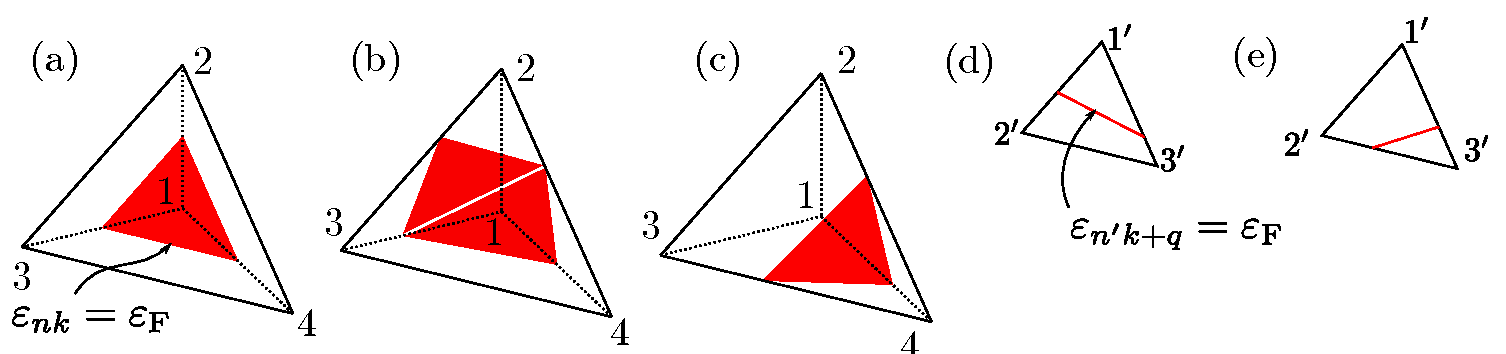
\includegraphics[width=16cm]{pic/elph_tetra.pdf}
  \caption{\label{fig_elph_tetra}
    How to divide a tetrahedron 
    in the case of $\epsilon_1 \leq \varepsilon_{\rm F} \leq \varepsilon_2$ (a), 
    $\varepsilon_2 \leq \varepsilon_{\rm F} \leq \varepsilon_3$ (b), and
    $\varepsilon_3 \leq \varepsilon_{\rm F} \leq \varepsilon_4$ (c).
  }
\end{figure}

\begin{itemize}

\item When $\varepsilon_1 \leq \varepsilon_{\rm F} \leq \varepsilon_2 \leq \varepsilon_3 \leq\varepsilon_4$
  [Fig. \ref{fig_elph_tetra}(a)], 

  \begin{align}
    F &= 
    \begin{pmatrix}
      a_{1 2} & a_{2 1} &       0 & 0 \\
      a_{1 3} &       0 & a_{3 1} & 0 \\
      a_{1 4} &       0 &       0 & a_{4 1}
    \end{pmatrix}, 
    \qquad
    \frac{S}{\nabla_k \varepsilon_k} = \frac{3 a_{2 1} a_{3 1} a_{4 1}}{\varepsilon_{\rm F} - \varepsilon_1}
  \end{align}
  
\item When $\varepsilon_1 \leq \varepsilon_2 \leq \varepsilon_{\rm F} \leq \varepsilon_3 \leq\varepsilon_4$
  [Fig. \ref{fig_elph_tetra}(b)], 
  %
  \begin{align}
    F &= 
    \begin{pmatrix}
      a_{1 3} &       0 & a_{3 1} & 0 \\
      a_{1 4} &       0 &       0 & a_{4 1} \\
            0 & a_{2 4} &       0 & a_{4 2}
    \end{pmatrix}, 
    \qquad
    \frac{S}{\nabla_k \varepsilon_k} = \frac{3 a_{3 1} a_{4 1} a_{2 4}}{\varepsilon_{\rm F} - \varepsilon_1}
  \end{align}
  
  \begin{align}
    F &= 
    \begin{pmatrix}
      a_{1 3} &       0 & a_{3 1} & 0 \\
            0 & a_{2 3} & a_{3 2} & 0 \\
            0 & a_{2 4} &       0 & a_{4 2}
    \end{pmatrix}, 
    \qquad
    \frac{S}{\nabla_k \varepsilon_k} = \frac{3 a_{2 3} a_{3 1} a_{4 2}}{\varepsilon_{\rm F} - \varepsilon_1}
  \end{align}

\item When $\varepsilon_1 \leq \varepsilon_2 \leq \varepsilon_3 \leq \varepsilon_{\rm F} \leq \varepsilon_4$
  [Fig. \ref{fig_elph_tetra}(c)], 

  \begin{align}
    F &= 
    \begin{pmatrix}
      a_{1 4} &       0 &       0 & a_{4 1} \\
      a_{1 3} & a_{2 4} &       0 & a_{4 2} \\
      a_{1 2} &       0 & a_{3 4} & a_{4 3}
    \end{pmatrix}, 
    \qquad
    \frac{S}{\nabla_k \varepsilon_k} = \frac{3 a_{1 4} a_{2 4} a_{3 4}}{\varepsilon_1 - \varepsilon_{\rm F}}
  \end{align}

\end{itemize}

Weights on each corners of the triangle are computed as follows
[($a'_{i j} \equiv (\varepsilon'_i - \varepsilon'_j)/(\varepsilon_{\rm F} - \varepsilon'_j)$)]:

\begin{itemize}

\item When $\varepsilon'_1 \leq \varepsilon_{\rm F} \leq \varepsilon'_2 \leq \varepsilon'_3$
  [Fig. \ref{fig_elph_tetra}(d)], 

  \begin{align}
    W'_1 = L (a'_{1 2} + a'_{1 3}), \qquad
    W'_2 = L a'_{2 1}, \qquad
    W'_3 = L a'_{3 1}, \qquad
    L \equiv \frac{a'_{2 1} a'_{3 1}}{\varepsilon_{\rm F} - \varepsilon'_{1}}
  \end{align}

\item When $\varepsilon'_1 \leq \varepsilon'_2 \leq \varepsilon_{\rm F} \leq \varepsilon'_3$
  [Fig. \ref{fig_elph_tetra}(e)], 

  \begin{align}
    W'_1 = L a'_{1 3}, \qquad
    W'_2 = L a'_{2 3}, \qquad
    W'_3 = L (a'_{3 1} + a'_{3 2}), \qquad
    L \equiv \frac{a'_{1 3} a'_{2 3}}{\varepsilon'_{3} - \varepsilon_{\rm F}} 
  \end{align}

\subsection{Eqn. (\ref{fml_goldenrule})}

In this case, we cut tetrahedra in the same manner to the case of 
\begin{align}
    \frac{\theta(\varepsilon_{\rm F} - \varepsilon_{k v \sigma})
      - \theta(\varepsilon_{\rm F} - \varepsilon_{k+q v' \sigma})}
         {\varepsilon_{k v \sigma} - \varepsilon_{k+q v' \sigma}}
         \theta(\varepsilon_{k+q v' \sigma} - \varepsilon_{k v \sigma})
\end{align}
in the DFPT calculation.
Then we evaluate $\delta(\varepsilon_{n' k+q} - \varepsilon_{n k} - \omega_{q \nu})$
in the trimmed tetrahedra.

\end{itemize}

\begin{thebibliography}{99}
  
\bibitem{DFPT-US}
  A. Dal Corso, Phys. Rev. B {\bf 64}, 235118 (2001).

\bibitem{opt_tetra}
  M. Kawamura, Phys. Rev. B {\bf 89}, 094515 (2014).
  
\end{thebibliography}


\end{document}
